% !TEX root = ../final-main.tex
\chapter{Future Work Recommendations}
\label{ch:future-work}

\section{Balancing Gate Leakage and Gate Control}

The oxide devices show that leakage reduction must be balanced against gate
control. The \SI{18}{\nano\metre} oxide layer strongly reduced gate leakage, but
the recessed oxide devices did not turn on within the measured voltage range.
This suggests that the dielectric thickness and recess depth were not matched
for the available gate-bias range.

For this reason, the oxide should not be treated as a simple process
improvement. A thinner oxide, a shallower recess, or an alternative dielectric
could reduce leakage while preserving stronger electrostatic access to the
channel. The important comparison is therefore not leakage alone, but the
combined behaviour of threshold voltage, turn-on voltage, gate leakage and
repeatability.

\section{Device Geometry}

Device geometry was a significant limitation in this work, particularly in
Iteration 1 where the recessed region did not fully control the available
source--drain current path. The device layout used in this project was selected
largely for practical reasons, since it was based on a mask already available
from cleanroom training. Although the gate design was improved in later
iterations, the resulting structure was still not ideal for studying a
gate-recess process, as the gate length and current path were not geometrically
uniform.

A Corbino-style circular HEMT would provide a cleaner test structure for this
type of investigation. In this geometry, the gate can surround the current path
between the drain and source more uniformly, reducing the possibility of current
bypassing the recessed region through unrecessed parts of the channel. This
would make the electrical response easier to interpret and would provide a more
suitable structure for engineering the relationship between recess depth, gate
control and threshold voltage.

\begin{figure}[htbp]
  \centering
  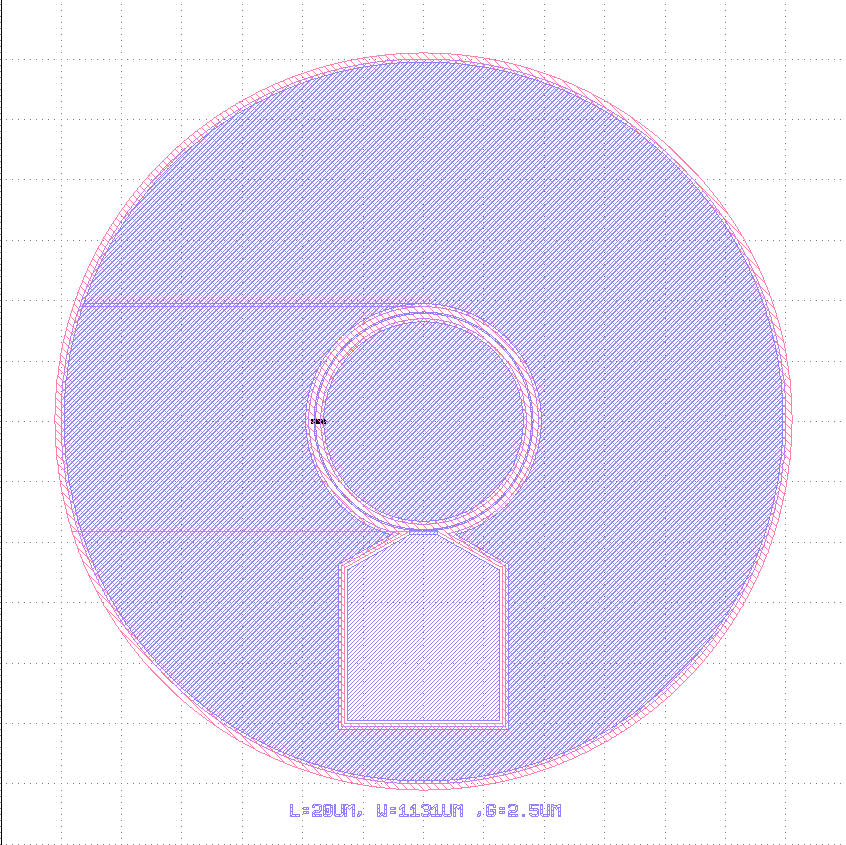
\includegraphics[width=0.33\linewidth]{figures/fabrication_images/recommendation/corbino_mask.png}
  \hspace{20mm}
  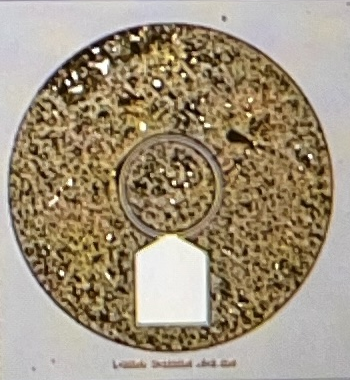
\includegraphics[width=0.33\linewidth]{figures/fabrication_images/recommendation/corbino.png}
  \caption{Proposed Corbino-style HEMT mask and device microscopy.}
  \label{fig:corbino-structure}
\end{figure}


\section{Etch Control}

The recess etch process is another clear area for improvement. Wet etching was
simple and accessible, but the results showed that it was highly sensitive to
mixing, timing, exposed area and agitation. A dry etch with laser endpoint
detection could offer improved depth control and repeatability, particularly
for recesses on the scale of only a few tens of nanometres \cite{Cadence2024}.

This recommendation carries a trade-off. Dry etching may improve depth
precision, but plasma damage or interface degradation could increase leakage or
reduce channel quality \cite{ZAPPE1993227}. A fair comparison between wet and
dry recessing should therefore consider threshold-voltage repeatability, gate
leakage, drain-source current and interface quality.
